\section{Dijeljeni kod i ulazni podaci}

\subsection{Čitanje i pisanje rezultata}

Kod u nastavku je dijeljeni kod tj. koristi se u oba algoritma. Sastoji se od metoda za čitanje datoteka s informacijama o oblacima točaka i metoda za spremanje transformacijskih matrica u datoteke. 

\begin{listing}[h!]
  \begin{minted}[frame=lines, linenos]{text}
typedef PointXYZ PT;
typedef PointCloud<PT> PointCloudType;
typedef IterativeClosestPoint<PT, PT, double> ICP;

PointCloudType::Ptr cloud_ref(new PointCloudType());
PointCloudType::Ptr cloud_target(new PointCloudType());
PointCloudType::Ptr cloud_reg(new PointCloudType());

PointCloudType::Ptr cloud_ref_f(new PointCloudType());
PointCloudType::Ptr cloud_target_f(new PointCloudType());

string root_point_clouds = "\\point_clouds\\";
string root_results = "\\icp_results\\";
  \end{minted}
  \caption{Generalizirani ICP - konstante}
  \label{coderef:gen_icp_const}
\end{listing}

U primjeru izvornoga koda \ref{coderef:gen_icp_const} su definirane konstante poput putanje za spremanje rezultata i putanje s ulaznim datotekama. Također su definirani tipovi točaka \mintinline{text}{PT} kao \mintinline{text}{PointXYZ} koje će algoritam koristit te sadrže samo x, y i z koordinate. Mogu se koristiti i drugi oblici točaka. Oblak točaka \mintinline{text}{PointCloudType} je definiran pomoću prethodne definicije točke. Naposljetku se definira tip \mintinline{text}{ICP} algoritma tj. s kojim timovima podataka radi. Definiran je pomoću uređene trojke \mintinline{text}{<PT, PT, double>} što znači da uspoređuje točke tipa \mintinline{text}{PT}, a rezultate u transformacijsku matricu zapisuje kao \mintinline{text}{double} vrijednosti.

Definirane su i varijable \mintinline{text}{cloud_ref} koja pokazuje na referentni skup točaka, \mintinline{text}{cloud_target} koja pokazuje na ciljni skup točakai \mintinline{text}{cloud_reg} koja pokazuje na skup točaka nakon poravnanja. Za algoritme koji koriste filrirane oblake točaka koriste se variable \mintinline{text}{cloud_ref_f} i \mintinline{text}{cloud_target_f}. One su tipa \mintinline{text}{boost::shared_ptr} te se kao takve predaju metodama kao pokazivači.

\begin{listing}[h!]
  \begin{minted}[frame=lines, linenos]{text}
ICP setupICP() {
 ICP icp;
 icp.setMaxCorrespondenceDistance(0.05);
 icp.setMaximumIterations(500);
 icp.setTransformationEpsilon(1e-8);
 icp.setEuclideanFitnessEpsilon(1);
 return icp;
}
  \end{minted}
  \caption{Generalizirani ICP - definicija ICP}
  \label{coderef:gen_icp_def}
\end{listing}
\pagebreak
U primjeru \ref{coderef:gen_icp_def} se definira ICP algoritam tako da mu se predaju uvjeti zaustavljanja te ostali parametri. Trenutno su zadana tri uvjeta zaustavljanja, a oni su:

\begin{enumerate}
  \item \mintinline{c++}{setMaxCorrespondenceDistance} - uzima u obzir samo točke unutar zadanoga promjera u metrima
  \item \mintinline{c++}{setMaximumIterations} - maksimalan broj iteracija prilikom estimacije matrice za neku točku
  \item \mintinline{c++}{setTransformationEpsilon} - maksimalna dozvoljena pogreška
\end{enumerate}

\begin{listing}[h!]
  \begin{minted}[frame=lines, linenos]{text}
vector<path> get_files() {
 vector<path> paths;
 path p(root_point_clouds);
 directory_iterator end_itr;
 for (directory_iterator itr(p); itr != end_itr; ++itr) {
  if (is_regular_file(itr->path())) {
   paths.push_back(itr->path());
  }
 }
 return paths;
}
  \end{minted}
  \caption{Generalizirani ICP - skupljanje datoteka}
  \label{coderef:gen_icp_collect_files}
\end{listing}
\pagebreak
Kod u primjeru \ref{coderef:gen_icp_collect_files} koristi metode biblioteke Boost za iteriranje datoteka sa skupovima točaka te vrača vektora s njihovim apsolutnim putanjama. Kod za stvaranje grafova je jednak bez obzira na korišteni algoritam. Grafovi su stvoreni pomoću jezika Kotlin i biblioteke XCharts. Podaci koji vizualiziraju su usporedbe stvarnih podataka tj. referentnih i podataka dobivenih pomoću algoritama. S obzirom da nam algoritmi kao izlaz daju samo transformacijske matrice, potrebno je nekako te matrice prikazati kao koordinate lokacija i kuteve rotacija.

\begin{listing}[h!]
  \begin{minted}[frame=lines, linenos]{text}
fun calculatePoints(
  icp: List<TransformMatrix>,
  realPoints: List<Point>)
: List<Point> {
    val calculatedPoints = mutableListOf(realPoints.first())
    realPoints.drop(1).forEachIndexed { index, _ ->
        val nrp = icp[index - 1] * realPoints[index - 1]
        calculatedPoints.add(nrp)
    }
    return calculatedPoints
}
  \end{minted}
  \caption{Generiranje estimiranih lokacija}
  \label{kotlin:gen_est_loc}
\end{listing}

Kod u primjeru \ref{kotlin:gen_est_loc} je prikazana funkcija za generiranje estimiranih točaka iz stvarnih točaka i transformacijskih matrica. Kao argumente metoda prima listu transformacijskih matrica \mintinline{text}{icp} te listu točaka koje predstavljaju referentne lokacija. Algoritam radi tako da se započinje od prve referentne točke te se na nju primjenjuje prva transformacijska matrica. Tako smo dobili sljedeću estimiranu točku. Nako toga se uzima sljedeća referentna točka te se ona množi s sljedećom transformacijskom matricom. N posljetku smo dobili niz estimiranih točaka koji sada možemo uspoređivati s referentnim nizom. S obzirom da je točka u obliku matrice 3x1, a transformacijska matrica ima oblik 3x3 oni se mogu pomnožiti pravilima množenja matrica. Tako se dobije sljedeća točka u nizu, a taj korak množenja je prikazan formulom \ref{eq:calc_next_point}.

\begin{equation}
  \begin{pmatrix}
  X_{n}\\
  Y_{n}\\
  Z_{n}\\
  1
  \end{pmatrix}
  =
  \begin{pmatrix}
    r_{11} & r_{12} & r_{13} & t_{x}\\
    r_{21} & r_{22} & r_{23} & t_{y}\\
    r_{31} & r_{32} & r_{33} & t_{z}\\
    0      & 0      & 0      & 1
  \end{pmatrix}
  \begin{pmatrix}
    X_{n-1}\\
    Y_{n-1}\\
    Z_{n-1}\\
    1
  \end{pmatrix}
  \label{eq:calc_next_point}
\end{equation}

\subsection{Ulazni podaci}

Za oba algoritma će se koristiti dva skupa podataka. Različiti parametri su korišteni prilikom skupljanja oba skupa iz simulatora.

Vizualizacije referentnih podataka za oba primjera kretanja vozila možemo vidjeti na sljedećim grafovima. Na njima svaka točka predstavlja jedno očitanje. Slika \ref{fig:gt1_lokacija} prikazuje graf lokacija vozila. Slika \ref{fig:gt1_lokacija_koord} pokazuje koordinate vozila u vremenu. Možemo vidjeti da se mijenjaju samo x i y koordinate zato što vozilo može samo skretati. Slika \ref{fig:gt1_rot_vr} valjanje, poniranje i skretanje oko statičnih osi vozila u vremenu. Također se može uoćiti da se samo skretanje mijenja zato što se vozilo ne može valjati niti ponirati. Slika \ref{fig:gt1_rot_kv} također pokazuje rotaciju vozila u vremenu ali predstavljenu u obliku kvaterniona. 

\subsubsection{Skup podataka A}
Prvi kup podataka se sastoji od 300 očitanja tj. postoji 300 datoteka sa skupovima točaka. Duljina trajanja te simulacije je 200 sekundi. Parametri koji su korišteni u python skripti za postavljanje lidar senzora su sljedeći:
\begin{enumerate}
  \item Maksimalna udaljenost laserske zrake je postavljena na 1500 cm tj. 15 metara
  \item Maksimalan skup točaka u jednome očitanju je postavljen na 600 000.
\end{enumerate}
\begin{figure}[H]
  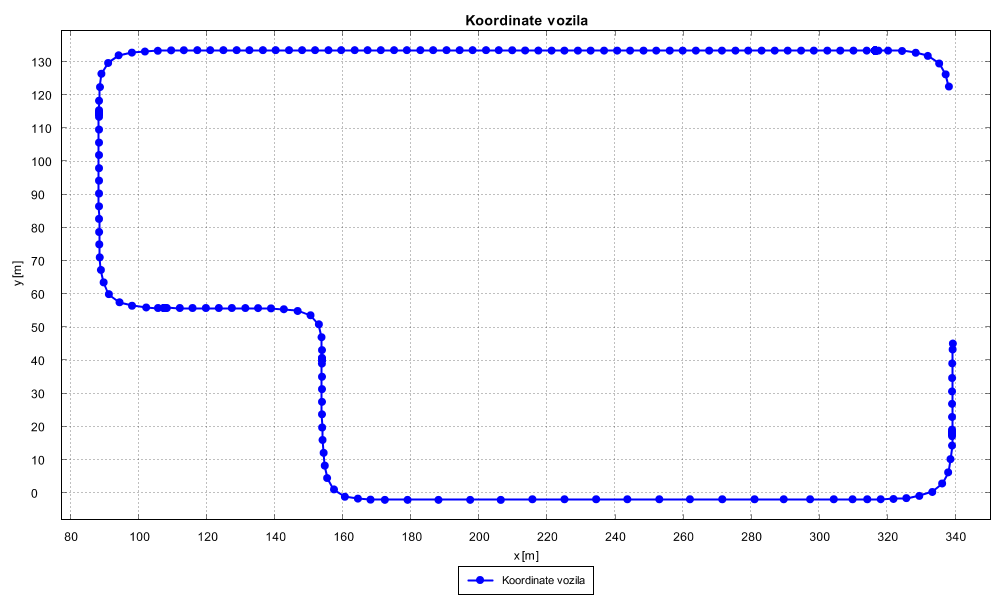
\includegraphics[scale=0.4]{images/koordinate1.png}
  \caption{Graf lokacije vozila}
  \label{fig:gt1_lokacija}
\end{figure}
\begin{figure}[H]
  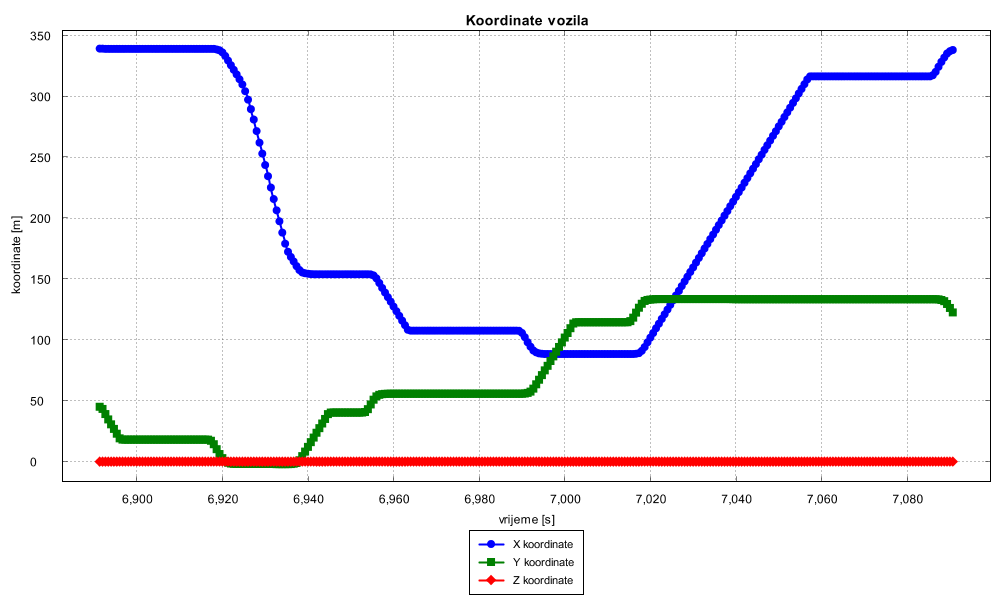
\includegraphics[scale=0.4]{images/koordinate_vrijeme1.png}
  \caption{Graf x, y i z koordinata vozila u vremenu}
  \label{fig:gt1_lokacija_koord}
\end{figure}
\begin{figure}[H]
  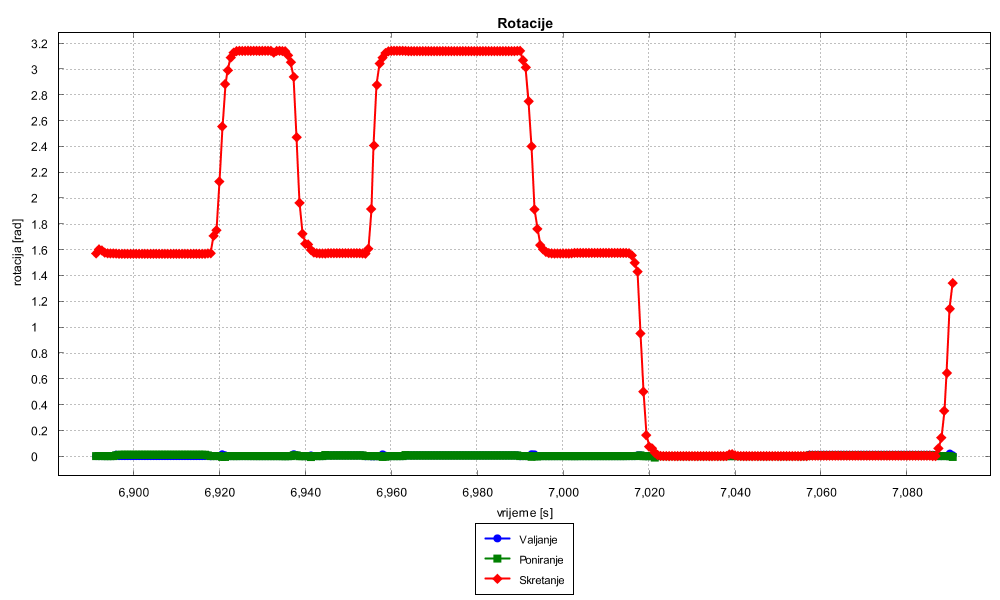
\includegraphics[scale=0.4]{images/rotacija_vrijeme1.png}
  \caption{Valjanje, skretanje i poniranje vozila u vremenu}
  \label{fig:gt1_rot_vr}
\end{figure}
\begin{figure}[H]
  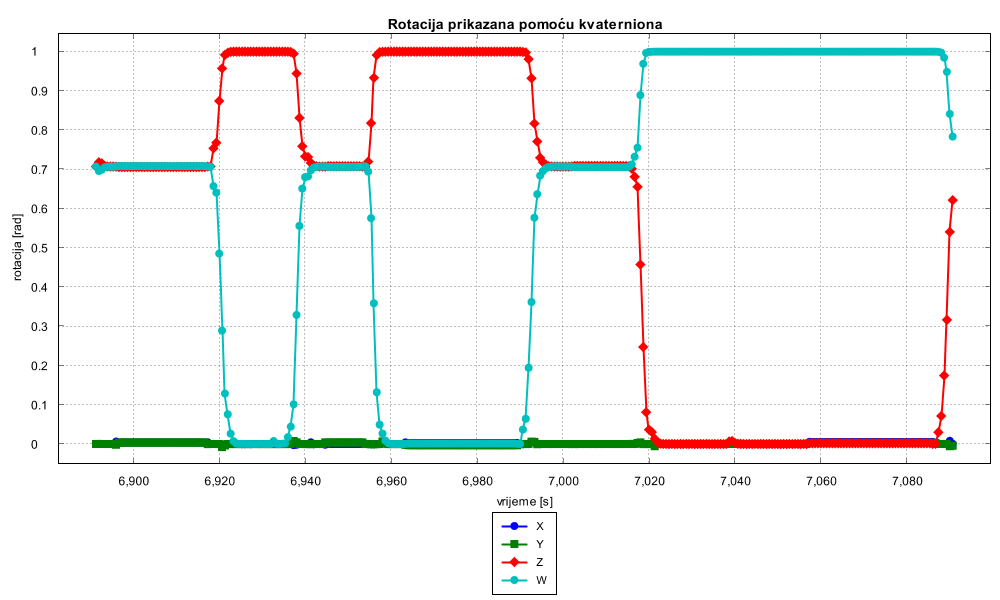
\includegraphics[scale=0.4]{images/rotacija_kvaterni1.png}
  \caption{Rotacija vozila u obliku kvaterniona}
  \label{fig:gt1_rot_kv}
\end{figure}

\newpage
\subsubsection{Skup podataka B}
Drugi skup podataka se sastoji od 600 očitanja tj. postoji 300 datoteka sa skupovima točaka. Duljina trajanja te simulacije je 80 sekundi. Parametri koji su korišteni u python skripti za postavljanje lidar senzora su sljedeći:
\begin{enumerate}
  \item Maksimalna udaljenost laserske zrake je postavljena na 2000 cm tj. 20 metara
  \item Maksimalan skup točaka u jednome očitanju je postavljen na 1 000 000.
\end{enumerate}
\begin{figure}[H]
  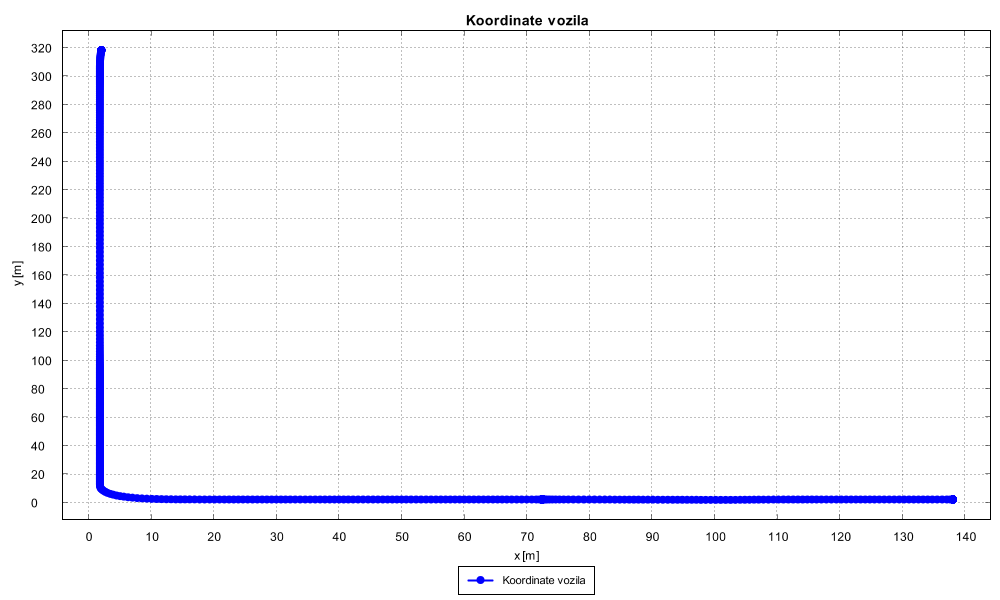
\includegraphics[scale=0.35]{images/koordinate2.png}
  \caption{Graf lokacije vozila}
  \label{fig:gt2_lokacija}
\end{figure}
\begin{figure}[H]
  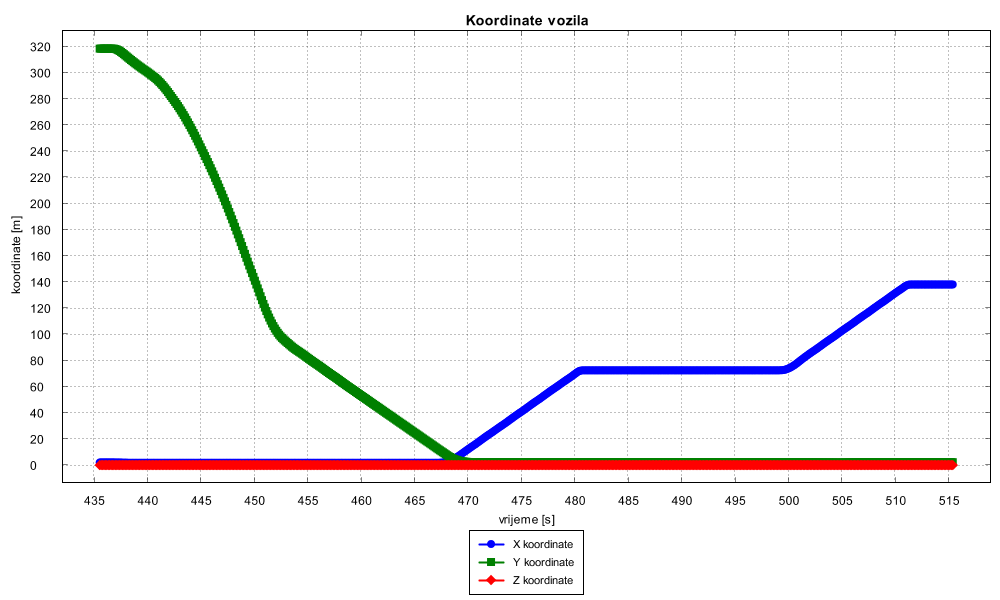
\includegraphics[scale=0.35]{images/koordinate_vrijeme2.png}
  \caption{Graf x, y i z koordinata vozila u vremenu}
  \label{fig:gt2_lokacija_koord}
\end{figure}
\begin{figure}[H]
  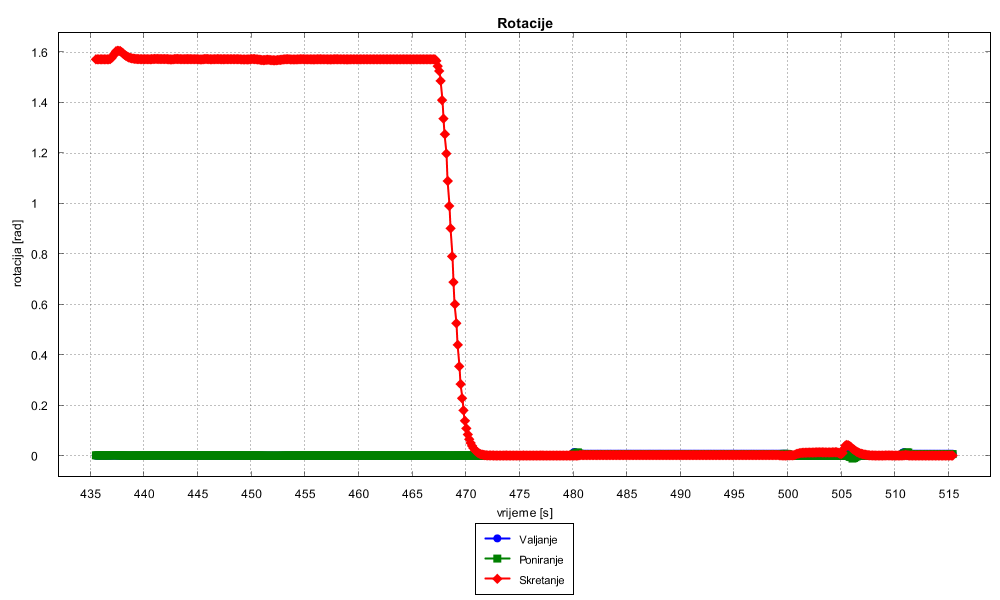
\includegraphics[scale=0.35]{images/rotacija_vrijeme2.png}
  \caption{Valjanje, skretanje i poniranje vozila u vremenu}
  \label{fig:gt2_rot_vr}
\end{figure}
\begin{figure}[H]
  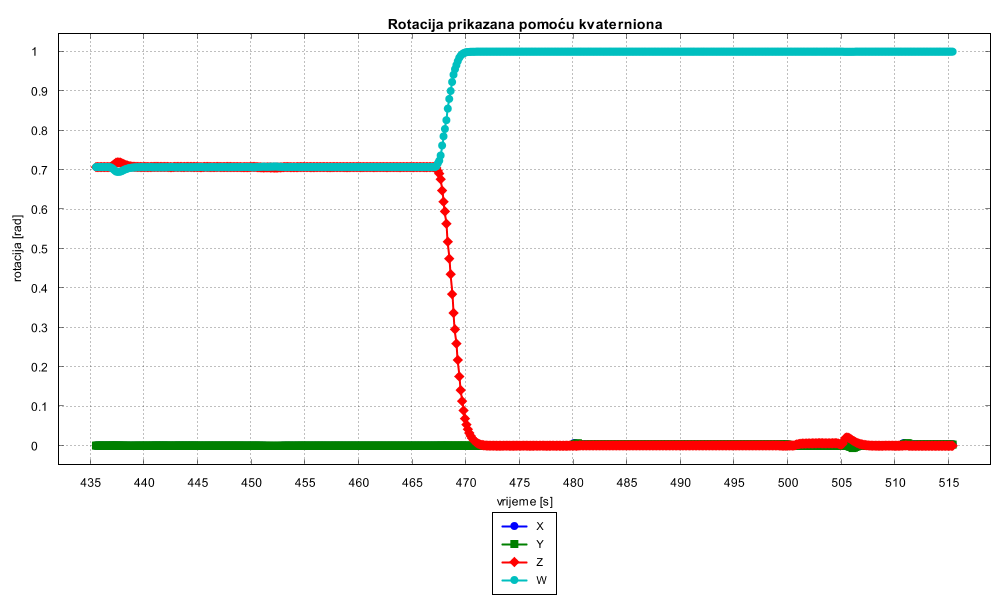
\includegraphics[scale=0.35]{images/rotacija_kvaterni2.png}
  \caption{Rotacija vozila u obliku kvaterniona}
  \label{fig:gt2_rot_kv}
\end{figure}
Prvi niz skupova točaka se skupljao u dužem periodu ali ima samo 300 skupova zato što se koristi svako 15 očitanje. Drugi niz skupova točaka ima 600 očitanja zato što se uzima svako očitanje. Također je drgi skup detaljniji od prvoga te se očekuju bolji rezultati algoritama. Duljinu puta možemo izračunati tako da pronađemo udaljenosti između dvije sljedne točke te ih zbrojimo. Tako dobivena udaljenost za referentni primjer A iznosi 662.3 metra, a za referentni primjer B iznosi 448.2 metra.